\documentclass{article}


% This file is a solution template for:
% 1 inch margins
\usepackage{fullpage}

\usepackage{booktabs}
\usepackage{longtable}

\usepackage{hyperref}
\usepackage{graphicx}
\usepackage{multicol}
\usepackage{subcaption}

% Add ability to resume enumeration environments with /begin{enumerate}[resume]
\usepackage{enumitem}

\usepackage{pgf}
\usepackage{tikz}
\usepackage{bodegraph}
\usepackage{circuitikz}
\usetikzlibrary{calc}
\usetikzlibrary{trees}
\usetikzlibrary{arrows}
\usetikzlibrary{shapes}
\usetikzlibrary{fadings}
\usetikzlibrary{positioning}
\usetikzlibrary{intersections}


\usepackage[english]{babel}
\usepackage[latin1]{inputenc}
\usepackage[T1]{fontenc}
% Or whatever. Note that the encoding and the font should match. If T1 does not look nice, try deleting the line with the fontenc.


\usepackage{listings}

\usepackage{amsmath}


\usepackage{xspace}
\newcommand{\Ohm}{$\Omega$\xspace}



\title{Comparators}

\begin{document}
\maketitle

So far, we have used op amps in their normal, linear mode, where they follow the op amp Golden Rules (no input current to either input, no voltage difference between the inputs). This week we look at comparators: specialty op amps which use positive feedback or no feedback.

\section{Comparators}
Sometimes, you want to use an op amp in its saturated mode --- where the output is pushed either as far positive or as far negative as it can go. This use changes the op amp from a linear device into a ``bistable'' device, that is, one that has only two possible output values.

The value of the output is based on a simple decision, made by the chip:
\begin{itemize}
\item If $V_+ > V_-$, then set the output to the positive rail.
\item If not, then set the output to the negative rail.
\end{itemize}
Such a circuit is called a comparator. This is the first step into the world of digital circuits where all output values are expressed as a series of ``yes'' or ``no'' answers.

\subsection{Positive Feedback}
We often refer to the $V_+$ voltage as the \emph{reference voltage} and connect the input to $V_-$. Comparators are supposed to determine:
\begin{itemize}
\item If the input ($V_-$) is less than the reference ($V_+$) then the output rails high. 
\item If the input ($V_-$) is greater than the reference ($V_+$) then the output rails low. 
\end{itemize}

However, when a comparator looks at a real input signal it will always be faced with some small variations in the signal that make it hard to determine which input is greater. Even worse, this electrical ``noise'' could drive your comparator through many transitions when you really wanted your signal to show only one transition. 

\begin{figure}
\begin{center}
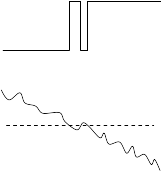
\includegraphics{pics/single_threshold}
\end{center}
\caption{A noisy signal on $V_-$ (bottom) generates multiple transitions (top) as it goes above and below the threshold on $V_+$ (dashed line).}
\label{fig:single_threshold}
\end{figure}

Figure~\ref{fig:single_threshold} shows how a little noise added to a slowly decreasing signal can cause multiple transitions in the output. The top curve shows the comparator output, while the bottom curve shows the $V_-$ input. The dashed line represents the $V_+$ input. When $V_-$ drops below the threshold (dashed line) the output changes state. When noise makes the input voltage briefly go back above the dashed curve the output ``bounces'' to low and back to high accordingly.

\begin{figure}
\begin{center}
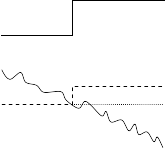
\includegraphics{pics/double_threshold}
\end{center}
\caption{When the output makes a transition (top), the reference level can be shifted (dashed) using positive feedback to prevent extra transitions as the input on $V_-$ (bottom) makes multiple transitions across the original reference voltage on $V_+$ (dotted line).}
\label{fig:double_threshold}
\end{figure}

The solution to this problem is to use positive feedback to simultaneously shift the reference voltage ($V_+$) as the output changes states. This is illustrated in Figure~\ref{fig:double_threshold}. If the shift is large enough, then the output will be less likely to bounce between the two output states during the transition. This shift, which is called a ``hysteresis'', depends on the design of the feedback network that ties $V_+$ to the output level.

\begin{figure}
\begin{center}
\begin{circuitikz}
\draw (0,0) node[op amp](opamp){};
\draw (opamp.-) to[short,-o] ++(0,0) node[left]{$V_{in}$};
\draw (opamp.+) node[circ](in1){} to[short] ++(0,-1.5) to[R,l=100\,k\Ohm] ++(2,0) -| (opamp.out) node[circ]{} to[R,l_=4.7\,k\Ohm,-o] ++(0,2) node[above]{5\,V};
\draw (opamp.out) to[short,-o] ++(0.5,0) node[right]{$V_{out}$};
\draw (in1) to[short] ++(-1.25,0) node[circ](in2){} to[R,l=50\,k\Ohm,-o] ++(0,2.5) node[above]{5\,V};
\draw (in2) to[R,l_=10\,k\Ohm] ++(0,-2.0) node[ground]{};
\end{circuitikz}
\end{center}
\caption{Comparator with hysteresis.}
\label{fig:comparator_with_hysteresis}
\end{figure}

An example of how this might work in an op amp implementation is shown in Figure~\ref{fig:comparator_with_hysteresis}. We will start by ignoring the positive feedback, and note that the $V_+$ input is tied to 0.83\,V via a voltage divider formed by a 10\,k\Ohm resistor and a 50\,k\Ohm resistor:
\begin{equation}
V_+ = 5\,\mbox{V} \cdot \frac{10\,\mbox{k\Ohm}}{50\,\mbox{k\Ohm} + 10\,\mbox{k\Ohm}} = 0.83\,\mbox{V}. \label{eqn:single_threshold}
\end{equation}
Now let's consider the effects of the feedback resistor. When the output is high, this places the 100\,k\Ohm resistor (ignore the 4.7\,k\Ohm for now) in parallel with the 50\,k\Ohm resistor so the reference voltage goes up to 1.16 V.
\begin{equation}
V_+ = 5\,\mbox{V} \cdot \frac{10\,\mbox{k\Ohm}}{33\,\mbox{k\Ohm} + 10\,\mbox{k\Ohm}} = 1.16\,\mbox{V}.
\end{equation}
When the output is low, the 100\,k\Ohm resistor is now in parallel with the 10\,k\Ohm resistor so the reference voltage goes down to 0.76 V.
\begin{equation}
V_+ = 5\,\mbox{V} \cdot \frac{9\,\mbox{k\Ohm}}{50\,\mbox{k\Ohm} + 9\,\mbox{k\Ohm}} = 0.76\,\mbox{V}.
\end{equation}
Therefore, this circuit's output will go from high to low when $V_-$ increases beyond 1.16\,V. The circuit's output will go from low to high when $V_-$ decreases below 0.76\,V. When $V_-$ is between 0.76\,V and 1.16\,V, the output will stay at its current value (either high or low). This memory of the past is why this type of feedback effect is called \emph{hysteresis} and is often represented as a plot of output voltage as a function of input voltage. The hysteresis in this case given by
\begin{equation}
1.16\,\mbox{V} - 0.76\,\mbox{V} = 0.40\,\mbox{V}.
\end{equation}

\begin{figure}
\begin{center}
\begin{tikzpicture}
\draw[->] (-4,0) -- (4,0) node[anchor=north] {$V_{in} - V_{ref}$};
\draw[->] (0,-1) -- (0,3) node[anchor=south] {$V_{out}$};
\draw[->] (-4,0.1) -- (-1,0.1) -- (-1,2.1) -- (4,2.1);
\draw[->] (4,1.9) -- (1,1.9) -- (1,-0.1) -- (-4,-0.1);
\end{tikzpicture}
\end{center}
\caption{A plot of $V_{out}$ vs.~$V_{in} - V_{ref}$ for a comparator with a positive feedback network.}
\label{fig:hysteresis}
\end{figure}

A plot of the reference voltage ($V_{out}$) vs.~the input voltage ($V_{in} - V_{ref}$) for a comparator with a positive feedback network (Figure~\ref{fig:hysteresis}). To make the two parts clear they have been slightly offset vertically. This type of plot is called a hysteresis plot. If there is an open box in the middle of the two paths then we say there is an input hysteresis. The hysteresis is defined as the difference between the two values of $V_{in}$ where there are transitions. 

This positive feedback circuit is called a \emph{Schmitt trigger}. A slightly better version can be made using two transistors but that's beyond the scope of this chapter.

\subsection{Comparators}
Commercial comparators are specialty op amps and come in a standard IC package. They are designed with the sole purpose of switching very quickly and do not have a number of the other good op amp qualities we have been exploiting in negative feedback circuits. The LM2903 and LM311 are the standard comparators that we will use in this week's lab.

\paragraph{Open-Collector Output}
Since comparators convert a linear signal into a digital signal, they are routinely used to connect two dissimilar electrical systems with different supply or reference voltages. Consequently, most standard comparators come designed to connect to any system you want to use. The output of a comparator is actually the collector input of a transistor switch (with ``open'' or ``closed'' states), rather than actual output voltages.  Note: in a regular op amp the output would be some form of push-pull stage.

\begin{figure}
\begin{center}
\begin{circuitikz}
\draw (0,0) node[op amp](opamp){};
\draw (1.75,0) node[npn](npn){};
\draw (opamp.-) to[short,-o] ++(0,0) node[left]{$V_{in}$};
\draw (opamp.+) to[short,-o] ++(0,0) node[left]{$V_{ref}$};
\draw (opamp.out) -- (npn.base);
\draw (npn.emitter) node[ground]{};
\draw (npn.collector) to[R,l_=4.7\,k\Ohm,-o] ++(0,1.5) node[above]{$V_{cc}$};
\end{circuitikz}
\end{center}
\caption{Equivalent circuit for an open collector output and a pull-up resistor.}
\label{fig:pull_up_resistor}
\end{figure}

When you use a comparator in a circuit, you usually connect the output to a voltage source via a \emph{pull-up resistor}, as shown in Figure~\ref{fig:pull_up_resistor}. When the comparator is in the high state, the switch will be open, no current will flow through the resistor. There will not be a voltage drop across the resistor, and hence the output will be pulled to the positive supply. When the comparator is in the low state, the switch will be closed, current will flow through the resistor. There will be a voltage drop across the resistor, and the output will be pulled to the lower supply level (ground in this case). The 4.7\,k\Ohm resistor in Figure~\ref{fig:comparator_with_hysteresis} is a pull-up resistor.

Even though the real open collector states are ``open'' and ``closed,'' they are still often called ``high'' and ``low'' in the assumption that you are using pull-up resistors.

\paragraph{Comparator Limitations}
Comparators typically have high gain at high frequencies and no phase compensation. Since comparators are designed to go all the way from the negative rail to the positive rail during transition, their data sheets list a transition delay time, which is the time to go from one rail to the other, instead of a slew rate.  For the LM2903 the transition time is roughly 1.5\,$\mu$s.

The most serious limitation for some comparators is that they will not allow a large voltage difference between $V_+$ and $V_-$. This difference is called the \emph{differential input voltage} and should be looked up on the data sheet before you design a circuit using a specific comparator.

Finally, another issue is that the input circuit's impedance changes as the output state changes.
 

\begin{figure}
\begin{center}
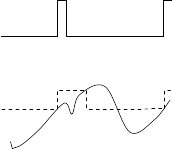
\includegraphics{pics/edge_trigger}
\end{center}
\caption{The output of the rising edge trigger sends out a pulse (top) when the input (bottom) rises past the threshold (dashed line). The output stays low when the output returns to below the threshold line. A hysteresis ensures that only one pulse is made per transition even in the presence of noise.}
\label{fig:edge_trigger}
\end{figure}

\paragraph{Edge Triggers}
A closely related class of circuits is triggers. A rising edge trigger will make a pulse (fast transition from low to high and back again) each time the input voltage rises past a particular threshold voltage. On the other hand, when the input voltage goes back below the threshold the output stays low. When the output is triggered, the threshold voltage is raised for a certain period of time to prevent multiple triggers.  After that time has elapsed, the threshold is lowered back to its normal value. This is called \emph{rearming} the trigger (Figure~\ref{fig:edge_trigger}). 

\section{Oscillators}
In many electronics applications it is useful to have a small function generator to synchronize various portions of a circuit or to insert time delays between different actions. This is called a \emph{clock signal}.

You should be used to this concept from a trip to a store shopping for PCs. The speed that it will perform individual operations (single core) is proportional to the clock speed. Therefore we know that 3.0\,GHz PC will be 10\% faster than a 2.7\,GHz PC. 

\begin{figure}
\begin{center}
\begin{circuitikz}
\draw (0,0) node[op amp](opamp){};
\draw (opamp.-) to[short] ++(0,1) node[circ](fb){} to[R,l=$R$] ++(2,0) -| (opamp.out);
\draw (fb) to[C,l_=$C$] ++(-1,0) node[ground]{};
\draw (opamp.out) node[circ]{} to[short] ++(0.5,0)  node[circ](out){} to[short,-o] ++(0.5,0) node[right]{$V_{out}$};
\draw (opamp.+) node[circ](in1){} to[short] ++(0,-1.5) to[R,l=100\,k\Ohm] ++(2,0) -| (out) to[R,l_=4.7\,k\Ohm,-o] ++(0,2) node[above]{5\,V};
\draw (in1) to[short] ++(-1.75,0) node[circ](in2){} to[R,l=100\,k\Ohm,-o] ++(0,2.5) node[above]{5\,V};
\draw (in2) to[R,l_=100\,k\Ohm] ++(0,-2.0) node[ground]{};
\end{circuitikz}
\end{center}
\caption{A square wave generator made using a relaxation oscillator.}
\label{fig:relaxation_oscillator}
\end{figure}

One simple way to make a clock signal is using positive feedback and a comparator to make a square wave generator. An example square wave generator is shown in Figure~\ref{fig:relaxation_oscillator}. The circuit is based on a comparator with hysteresis.  The comparator is assumed to be powered by 0\,V and +5\,V. The divider in this example defines the transition levels to be $V_+/3$ and $2V_+/3$. 

The wrinkle here is that the output is connected to the reference voltage through an $RC$ circuit. After the output switches state, the capacitor gets charged by the voltage at the output.  When the charge on the capacitor gets higher than $2V_+/3$, the hysteresis causes the output to change states and the capacitor gets discharged. When the charge on the capacitor gets lower than $V_+/3$ then the output changes states again.  This process repeats forever and the resulting output is a square wave. The square wave will have the period given by roughly $2 RC \ln 2$. 

These kinds of circuits are called \emph{relaxation oscillators} or \emph{$RC$ oscillators}. They generally work well for frequencies from around 1\,kHz to 1\,MHz. When designing an oscillator, make sure that $R$ is significantly larger than the pull-up resistor or the output will be asymmetric. (Can you to figure out why?)

In precision applications the simple $RC$ oscillator would be replaced by a vibrating crystal. Vibrating crystals are available as precision oscillators with a wide range of frequencies. Suggested designs for using crystals with comparators are available in the data sheets.


\pagebreak

\section{Design Exercises}

\begin{enumerate}
\item Design a comparator that will switch when the input signal crosses $+2.5$\,V with no hysteresis (as in equation~\ref{eqn:single_threshold}).
 
\item Modify the design of your comparator with a positive feedback network to add a total hysteresis of approximately 0.2\,V.

\item \label{ex:relaxation_oscillator} Design a relaxation oscillator with 10\,Hz frequency. Use resistor and capacitor values in the same range as those found in the electronics lab.

\item (Bonus) If you run design exercise~\ref{ex:relaxation_oscillator} in 5Spice, then you will notice that the square wave is not symmetric (i.e. ``high'' time is longer than the ``low'' time). Modify the circuit so that you can make the square wave symmetric.
\end{enumerate}

\section{Lab: Comparators and Oscillators}

\begin{enumerate}
\item Connect a LM2903 comparator to measure where a sine wave crosses $+2.5$\,V, with no feedback. Read the data sheet to see the power requirement for your comparator, double check with your instructor. Remember that the output must use a ``pull-up'' resistor. Use a 4.7\,k\Ohm pull up resistor tied to +5\,V. Observe and characterize its output when driven by a 1 kHz sine wave with a 1\,V amplitude and a DC offset larger than +1.5 V.

Add positive feedback to your comparator to generate a total hysteresis of 0.2\,V and observe its effect.

\item Build a square wave oscillator with 10\,Hz frequency that drives a green or red LED.  Examine the voltage across the capacitor and the output voltage on your scope at the same time to understand the switching structure. Make sure that on and off time is approximately the same.

\item Build the power source which converts +15\,V voltage to +5\,V using a +5\,V voltage regulator (MC7805, see datasheet for more details).  Swing input voltage and see at what values you stop receiving +5\,V. 

\item Make sure that your blinker is still working with the above power source.
\end{enumerate}

\end{document}
